\documentclass[10pt,]{beamer}
\hypersetup{pdfpagemode=FullScreen}

\usepackage{pgfpages}
\usepackage[style=authortitle,backend=bibtex]{biblatex}
% \bibliography{Bibliography}
\addbibresource{Bibliography.bib}

\mode<handout>{%
    \pgfpagesuselayout{4 on 1}[a4paper,landscape] 
    %\setbeameroption{show notes}
    \setbeamercolor{note page}{bg=white}
}

\usepackage[]{amsmath}
\usepackage{amsthm,amssymb,amsfonts}
\usepackage{graphicx,xfrac,mathrsfs,subcaption}
\usepackage{tikz,pgfplots}
\usepackage{tikzpagenodes}
\usepackage{multicol,multirow}
\usepackage{algorithm2e}
\usepackage{algorithmic}

\usetikzlibrary{positioning,automata}
\usetikzlibrary{matrix}
\usetikzlibrary{arrows,shapes}
\usetikzlibrary{trees}
\usetikzlibrary{backgrounds}
\usetikzlibrary{shapes.geometric}
\usetikzlibrary{calc,shapes.callouts,shapes.arrows}
\usetikzlibrary{graphs}
\usetikzlibrary{positioning, arrows}
\usetikzlibrary{fit}

\tikzset{onslide/.code args={<#1>#2}{%
  \only<#1>{\pgfkeysalso{#2}}
}}


%%%%%%%%%%%%%%%%%%%%%%%%%%%%
%%%%%%%%%%%%%%%%%%%%%%%%%%%%
%%%%% long and short versions
\newcommand{\extra}[1]{}
\newcommand{\short}[1]{#1}

% Custom colors
\definecolor{darkGreen}{HTML}{023618}
\definecolor{darkPurple}{HTML}{1C0221}
\definecolor{textGreen}{HTML}{628B48}
\definecolor{claimGreen}{HTML}{AF125A}

% Custom theorem styles
\makeatletter
\def\th@conjectureStyle{%
    \normalfont % body font
    \setbeamercolor{block title example}{bg=darkGreen,fg=white}
    \setbeamercolor{block body example}{bg=darkGreen!20,fg=black}
    \def\inserttheoremblockenv{exampleblock}
  }
\makeatother
\theoremstyle{conjectureStyle}
\newtheorem*{conjecture}{Conjecture}

\makeatletter
\def\th@notationStyle{%
    \normalfont % body font
    \setbeamercolor{block title example}{bg=darkPurple,fg=white}
    \setbeamercolor{block body example}{bg=darkPurple!20,fg=black}
    \def\inserttheoremblockenv{exampleblock}
  }
\makeatother
\theoremstyle{notationStyle}
\newtheorem*{notation}{Notation}

\makeatletter
\def\th@claimStyle{%
    \normalfont % body font
    \setbeamercolor{block title example}{bg=claimGreen,fg=white}
    \setbeamercolor{block body example}{bg=claimGreen!20,fg=black}
    \def\inserttheoremblockenv{exampleblock}
  }
\makeatother
\theoremstyle{claimStyle}
\newtheorem*{claim}{Claim}

\usetheme{Boadilla}
\makeatother
\setbeamertemplate{footline}
{
	\leavevmode%
	\hbox{%
	\begin{beamercolorbox}[wd=.4\paperwidth,ht=2.25ex,dp=1ex,center]{author in head/foot}%
		\usebeamerfont{author in head/foot}\insertshortauthor
	\end{beamercolorbox}%
	\begin{beamercolorbox}[wd=.6\paperwidth,ht=2.25ex,dp=1ex,center]{title in head/foot}%
		\usebeamerfont{title in head/foot}\insertshorttitle\hspace*{3em}
		\insertframenumber{} / \inserttotalframenumber\hspace*{1ex}
	\end{beamercolorbox}}%
	\vskip0pt%
}
\makeatletter

\setbeamertemplate{navigation symbols}{}
\title[HK-property | Perfect Binary Trees]{Exploring perfect binary trees with relation to the HK-property}
\subtitle{MXML Presentation} %This is where you can specify the conference name or presentation venue
\author[A.M]{Atishaya Maharjan}
\date{\today}

\begin{document}
\parskip = \baselineskip

\begin{frame} %Title page
    \titlepage
\end{frame}

\begin{frame}{Outline}
    \tableofcontents
\end{frame}

\section{EKR Theorem}
\begin{frame}\frametitle{EKR Theorem}
    The \textbf{Erd\H{o}s-Ko-Rado} theorem limits the number of sets in an intersecting family.
    \begin{theorem}[EKR Theorem]
        \footcite{Erds1961INTERSECTIONTF} If $\mathcal{F}$ is an intersecting family of $k$-subsets of an $n$-set (cardinality of the set is $n$), then
        \begin{itemize}
            \item $|\mathcal{F}| \leq \binom{n - 1}{k - 1}$
            \item If equality holds, $\mathcal{F}$ consists of the $k$-subsets that contain $i$, for some $i$ in the $n$-set.
        \end{itemize}
    \end{theorem}
\end{frame}

\section{HK-property}
\begin{frame}\frametitle{HK-property}
    \begin{definition}[Cocliques]
        \begin{itemize}
            \item A \textbf{coclique} in a graph is a set of vertices such that no two vertices in the set are adjacent.
            \item The maximum size of a coclique in a graph is called the \textbf{maximum coclique} of the graph. For a graph $G$, it is denoted by $\alpha(G)$.
        \end{itemize}
    \end{definition}
    \pause

    \begin{definition}[Stars and Stars Center]
        \begin{itemize}
            \item In a graph $G$, the set of all cocliques of a fixed size $k$, including a fixed vertex $v$ is called a star centered at $v$.
            \item It is denoted by $\mathcal{I}^k_G(v)$.
        \end{itemize}
    \end{definition}
    \pause

    \begin{definition}[k-EKR graph]
        Let $\mathcal{F}$ be a family of cocliques of fixed size $k$ in a graph G such that any two sets in $\mathcal{F}$ have a non-empty intersection. Then, there exists a vertex $v$ such that $|\mathcal{F}| \leq \mathcal{I}^k_G(v)$.
    \end{definition}
\end{frame}

\begin{frame}\frametitle{HK-property}
    Studying the EKR theorem, \footcite{MR2763040} Hurlbert and Kamat made the following conjecture:
    \begin{conjecture}[HK-Property]
        For any $k \geq 1$ and any tree $T$, there exists a leaf $l$ of $T$ such that $|\mathcal{I}^k_T(v)| \leq |\mathcal{I}^k_T(l)|$ for each $v \in V(T)$.
    \end{conjecture}
\end{frame}

\begin{frame}\frametitle{HK-property}
    \begin{itemize}
        \item The HK-property was proven for $k \leq 4$, but the conjecture was shown to be false.\footcite{MR2523796} \footcite{MR3612439} \footcite{MR3271819}
    \end{itemize}

    \begin{figure}
        \centering
        \begin{tikzpicture}[scale=0.7,level distance=2cm,
                level 1/.style={sibling distance=8cm},
                level 2/.style={sibling distance=4cm},
                level 3/.style={sibling distance=2cm},
                every node/.style={circle, draw, fill=white, minimum size=1.75em},]
            \node (v11) {$v_0$}
            child {node (v21) {$v_1$}
                    child {node  {}
                            child {node {}}
                        }
                    child {node (v32) {}
                            child {node {}}
                        }
                }
            child {node (v22) {$v_2$}
                    child {node (v33) {}
                            child {node {}}
                        }
                    child {node (v34) {}
                            child {node {}}
                        }
                };
        \end{tikzpicture}
        \caption*{Figure 1: The largest k-star for $k \geq 5$ is centered at $v_0$}
    \end{figure}
\end{frame}

\begin{frame}\frametitle{Some graphs that DO satisfy the HK-property \footcite{MR2763040}}
    \textbf{Caterpillars:}
    \centering
    \begin{figure}
        \centering
        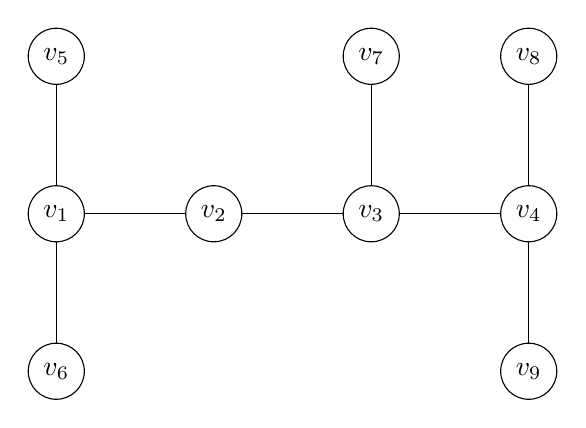
\begin{tikzpicture}[every node/.style={circle, draw, fill=white, minimum size=1.75em}]
            % Draw the path (spine)
            \node (v1) at (0,0) {$v_1$};
            \node (v2) at (2,0) {$v_2$};
            \node (v3) at (4,0) {$v_3$};
            \node (v4) at (6,0) {$v_4$};
            \draw (v1) -- (v2) -- (v3) -- (v4);

            % Draw the leaves
            \node (v5) at (0,2) {$v_5$};
            \node (v6) at (0,-2) {$v_6$};  % New vertex attached to v1
            \node (v7) at (4,2) {$v_7$};
            \node (v8) at (6,2) {$v_8$};
            \node (v9) at (6,-2) {$v_9$};  % New vertex attached to v4
            \draw (v1) -- (v5);
            \draw (v1) -- (v6);  % Edge to the new vertex
            \draw (v3) -- (v7);
            \draw (v4) -- (v8);
            \draw (v4) -- (v9);  % Edge to the new vertex
        \end{tikzpicture}
        \caption*{Figure: A caterpillar}
    \end{figure}
\end{frame}



\begin{frame}\frametitle{Some graphs that DO satisfy the HK-property \footcite{MR2763040}}
    \textbf{Spiders:}
    \centering
    \begin{figure}
        \centering
        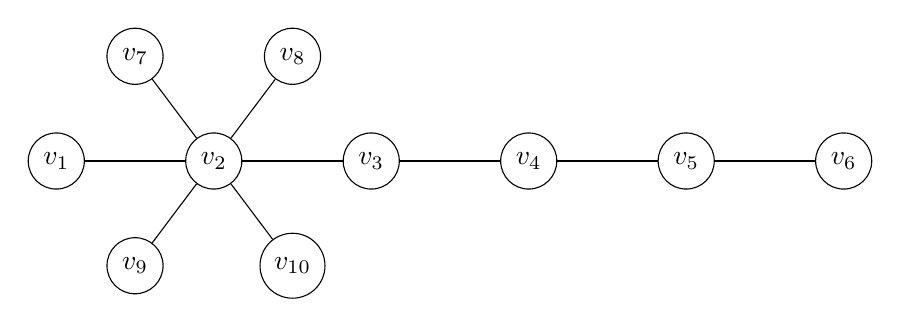
\begin{tikzpicture}[every node/.style={circle, draw, fill=white, minimum size=1.75em}]
            % Draw the path (spine)
            \node (v1) at (0,0) {$v_1$};
            \node (v2) at (2,0) {$v_2$};
            \node (v3) at (4,0) {$v_3$};
            \node (v4) at (6,0) {$v_4$};
            \node (v5) at (8,0) {$v_5$};
            \node (v6) at (10,0) {$v_6$};
            \draw (v1) -- (v2) -- (v3) -- (v4) -- (v5) -- (v6);

            % Draw the leaves
            \node (v7) at (1,1.33) {$v_7$};
            \node (v8) at (3,1.33) {$v_8$};
            \node (v9) at (1,-1.33) {$v_9$};
            \node (v10) at (3,-1.33) {$v_{10}$};
            \draw (v2) -- (v7);
            \draw (v2) -- (v8);
            \draw (v2) -- (v9);
            \draw (v2) -- (v10);
        \end{tikzpicture}
        \caption*{Figure: A Spider}
    \end{figure}
\end{frame}

\begin{frame}\frametitle{Some graphs that DO satisfy the HK-property \footcite{MR2763040}}
    \textbf{Lobsters*:}
    \centering
    \begin{figure}
        \centering
        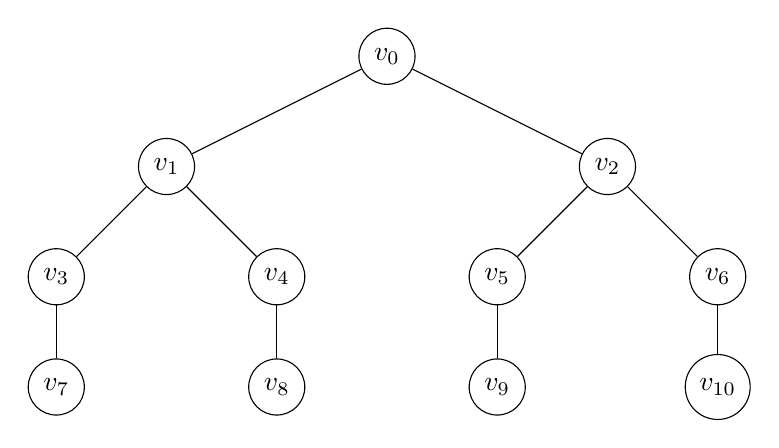
\begin{tikzpicture}[scale=0.7,level distance=2cm,
                level 1/.style={sibling distance=8cm},
                level 2/.style={sibling distance=4cm},
                level 3/.style={sibling distance=2cm},
                every node/.style={circle, draw, fill=white, minimum size=1.75em},]
            \node (v11) {$v_0$}
            child {node (v21) {$v_1$}
                    child {node  {$v_3$}
                            child {node {$v_7$}}
                        }
                    child {node (v32) {$v_4$}
                            child {node {$v_8$}}
                        }
                }
            child {node (v22) {$v_2$}
                    child {node (v33) {$v_5$}
                            child {node {$v_9$}}
                        }
                    child {node (v34) {$v_6$}
                            child {node {$v_{10}$}}
                        }
                };
        \end{tikzpicture}
        \caption*{Figure: A Lobster}
    \end{figure}a
\end{frame}

\section{Perfect Binary Trees}
\begin{frame}\frametitle{Perfect Binary Tree}
    \textbf{Perfect Binary Tree:}
    \centering
    \begin{figure}
        \centering
        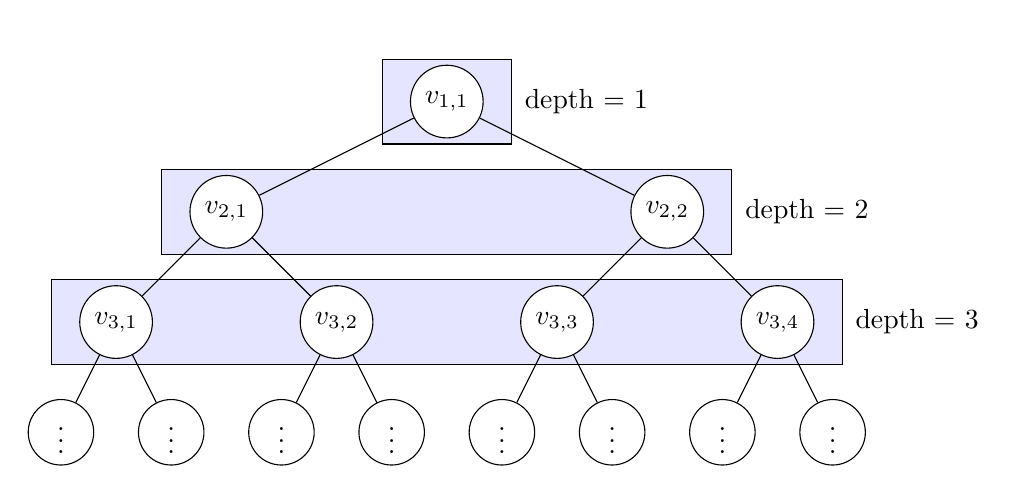
\begin{tikzpicture}[scale=0.7,level distance=2cm,
                level 1/.style={sibling distance=8cm},
                level 2/.style={sibling distance=4cm},
                level 3/.style={sibling distance=2cm},
                every node/.style={circle, draw, fill=white}]
            \node (v11) {$v_{1,1}$}
            child {node (v21) {$v_{2,1}$}
                    child {node (v31) {$v_{3,1}$}
                            child {node {$\vdots$}}
                            child {node {$\vdots$}}
                        }
                    child {node (v32) {$v_{3,2}$}
                            child {node {$\vdots$}}
                            child {node {$\vdots$}}
                        }
                }
            child {node (v22) {$v_{2,2}$}
                    child {node (v33) {$v_{3,3}$}
                            child {node {$\vdots$}}
                            child {node {$\vdots$}}
                        }
                    child {node (v34) {$v_{3,4}$}
                            child {node {$\vdots$}}
                            child {node {$\vdots$}}
                        }
                };

            \begin{scope}[on background layer]
                \node[draw,rectangle,fit=(v11),inner xsep=10pt, inner ysep=2pt, fill=blue!10, label=right:{depth = 1}] {};
                \node[draw,rectangle,fit=(v21) (v22),inner xsep=10pt, inner ysep=2pt, fill=blue!10, label=right:{depth = 2}] {};
                \node[draw,rectangle,fit=(v31) (v32) (v33) (v34),inner xsep=10pt, inner ysep=2pt, fill=blue!10, label=right:{depth = 3}] {};
            \end{scope}
        \end{tikzpicture}
    \end{figure}
\end{frame}



\section{Does a perfect binary tree satisfy the HK property?}
\begin{frame}\frametitle{Does a perfect binary tree satisfy the HK property?}
    \begin{enumerate}[<+->]
        \setlength\itemsep{2em}
        \item At least partially.
        \item The lobster almost satisfies the HK property and the perfect binary tree has a close relation to the lobster.
        \item In addition, the perfect binary tree is very symmetric and has a lot of structure that we can maniputlate.
    \end{enumerate}
\end{frame}

\section{Algorithmic Approach and Computer Verification}
\begin{frame}\frametitle{Using an enumeration approach with computer algorithms to verify the results}
    Before we proceed with proving anything, it would be helpful to first verify some results and get some data using computer algorithms.
\end{frame}

\begin{frame}\frametitle{Using an enumeration approach with computer algorithms to verify the results}
    \begin{algorithm}[H]
        \KwData{A perfect binary tree graph $T$}
        \KwResult{All cocliques of $T$}

        \SetKwFunction{FMain}{enumerate\_cocliques}

        \SetKwProg{Fn}{Function}{:}{}
        \Fn{\FMain{$T$}}{
            $cocliques \gets []$\;
            $cocliques$.append($\emptyset$)\;
            \For{$vertex$ in $T$}{
                $new\_cocliques \gets []$\;
                \For{$coclique$ in $cocliques$}{
                    \For{$neighbor$ in $vertex.neighbors$}{
                        \If{$neighbor \not\in coclique$}{
                            $new\_coclique \gets coclique \cup \{neighbor\}$\;
                            $new\_cocliques$.append($new\_coclique$)\;
                        }
                    }
                }
                $cocliques \gets new\_cocliques$\;
            }
            \Return{$cocliques$}
        }
    \end{algorithm}
\end{frame}

\begin{frame}\frametitle{Using an enumeration approach with computer algorithms to verify the results}
    \begin{enumerate}[<+->]
        \item The results do indeed verify that the HK-property holds for perfect binary trees of depth 5. With the pattern, it might hold for any depth perfect binary tree.
        \item It does also show us that all the leaves are included in the maximum coclique.
        \item However, patterns have a history of misleading mathematicians and as such, a proof is needed.
    \end{enumerate}
\end{frame}

\section{Inductive Approach}
\begin{frame}\frametitle{Inductive Approach}
    We can conjecture a formula for the maximum coclique of a perfect binary tree of depth $d$:

    \begin{conjecture}
        For any perfect binary tree $T$ of depth $d$, the maximum coclique $\alpha(T)$ is given by
        \begin{align*}
            \alpha(T) = \sum_{i= 0}^{\left\lfloor\frac{d}{2}\right\rfloor} 2^{d - 2i}
        \end{align*}

        Furthermore, the maximum coclique is unique.
    \end{conjecture}

    This is still a work in progress, but we believe that we can give an inductive proof for this conjecture by inducting on $d$.
\end{frame}

\begin{frame}\frametitle{Inductive Approach}
    If the previous conjecture holds, then we claim that:

    \begin{claim}
        There is a unique maximum coclique set that contains all the leaves.
    \end{claim}

    Then from the claim and all the observations, we can conjecture the following:

    \begin{conjecture}
        Let $T$ be a perfect binary tree of depth $d$. Let $r$ be the root of $T$. Then, for all possible values of $d$ and $k$, there exists a leaf $l$ of $T$ such that $|\mathcal{I}^k_T(v)| \leq |\mathcal{I}^k_T(l)|$ for each $v \in V\setminus{r}$.
    \end{conjecture}

    Which is partially the HK conjecture. Note that this is the exact statement for the HK conjecture for lobsters given by \footcite{MR4245360} Estrugo and Pastine.
\end{frame}

\section{Open Questions and Future Work}
\begin{frame}\frametitle{Open Questions and Future work}
    Note that a perfect binary tree is just a specific case for a perfect $k$-nary tree. So, we can most likely generalize the results for perfect $k$-nary trees to show that they satisfy a partial HK-property, similar to those of the binary tree.

    In addition, we can also investigate the HK-property for other types of binary trees (Full, Complete, Normal, etc) and see if they satisfy the HK-property.
\end{frame}



%%%%%%%%%%%%%%%%%%%%%%%%%%%%%%%%%%%%%%%%%%%%%%%%%%%%%%%%%%%%%%%%%%%%%%
%%%%%%%%%%%%%%%%%%%%%%%%%%%%%%%%%%%%%%%%%%%%%%%%%%%%%%%%%%%%%%%%%%%%%%  
%%%%%%%%%%%%%%%%%%%%%%%%%%%%%%%%%%%%%%%%%%%%%%%%%%%%%%%%%%%%%%%%%%%%%%
\begin{frame}\frametitle{Thank You!}
    \begin{center}
        Thank you for listening!\\
    \end{center}
\end{frame}
%%%%%%%%%%%%%%%%%%%%%%%%%%%%%%%%%%%%%%%%%%%%%%%%%%%%%%%%%%%%%%%%%%%%%%
%%%%%%%%%%%%%%%%%%%%%%%%%%%%%%%%%%%%%%%%%%%%%%%%%%%%%%%%%%%%%%%%%%%%%%  
%%%%%%%%%%%%%%%%%%%%%%%%%%%%%%%%%%%%%%%%%%%%%%%%%%%%%%%%%%%%%%%%%%%%%%

\end{document}
